
%% bare_conf.tex
%% V1.3
%% 2007/01/11
%% by Michael Shell
%% See:
%% http://www.michaelshell.org/
%% for current contact information.
%%
%% This is a skeleton file demonstrating the use of IEEEtran.cls
%% (requires IEEEtran.cls version 1.7 or later) with an IEEE conference paper.
%%
%% Support sites:
%% http://www.michaelshell.org/tex/ieeetran/
%% http://www.ctan.org/tex-archive/macros/latex/contrib/IEEEtran/
%% and
%% http://www.ieee.org/

%%*************************************************************************
%% Legal Notice:
%% This code is offered as-is without any warranty either expressed or
%% implied; without even the implied warranty of MERCHANTABILITY or
%% FITNESS FOR A PARTICULAR PURPOSE! 
%% User assumes all risk.
%% In no event shall IEEE or any contributor to this code be liable for
%% any damages or losses, including, but not limited to, incidental,
%% consequential, or any other damages, resulting from the use or misuse
%% of any information contained here.
%%
%% All comments are the opinions of their respective authors and are not
%% necessarily endorsed by the IEEE.
%%
%% This work is distributed under the LaTeX Project Public License (LPPL)
%% ( http://www.latex-project.org/ ) version 1.3, and may be freely used,
%% distributed and modified. A copy of the LPPL, version 1.3, is included
%% in the base LaTeX documentation of all distributions of LaTeX released
%% 2003/12/01 or later.
%% Retain all contribution notices and credits.
%% ** Modified files should be clearly indicated as such, including  **
%% ** renaming them and changing author support contact information. **
%%
%% File list of work: IEEEtran.cls, IEEEtran_HOWTO.pdf, bare_adv.tex,
%%                    bare_conf.tex, bare_jrnl.tex, bare_jrnl_compsoc.tex
%%*************************************************************************

% *** Authors should verify (and, if needed, correct) their LaTeX system  ***
% *** with the testflow diagnostic prior to trusting their LaTeX platform ***
% *** with production work. IEEE's font choices can trigger bugs that do  ***
% *** not appear when using other class files.                            ***
% The testflow support page is at:
% http://www.michaelshell.org/tex/testflow/



% Note that the a4paper option is mainly intended so that authors in
% countries using A4 can easily print to A4 and see how their papers will
% look in print - the typesetting of the document will not typically be
% affected with changes in paper size (but the bottom and side margins will).
% Use the testflow package mentioned above to verify correct handling of
% both paper sizes by the user's LaTeX system.
%
% Also note that the "draftcls" or "draftclsnofoot", not "draft", option
% should be used if it is desired that the figures are to be displayed in
% draft mode.
%
\documentclass[conference]{IEEEtran}
% Add the compsoc option for Computer Society conferences.
%
% If IEEEtran.cls has not been installed into the LaTeX system files,
% manually specify the path to it like:
% \documentclass[conference]{../sty/IEEEtran}





% Some very useful LaTeX packages include:
% (uncomment the ones you want to load)


% *** MISC UTILITY PACKAGES ***
%
%\usepackage{ifpdf}
% Heiko Oberdiek's ifpdf.sty is very useful if you need conditional
% compilation based on whether the output is pdf or dvi.
% usage:
% \ifpdf
%   % pdf code
% \else
%   % dvi code
% \fi
% The latest version of ifpdf.sty can be obtained from:
% http://www.ctan.org/tex-archive/macros/latex/contrib/oberdiek/
% Also, note that IEEEtran.cls V1.7 and later provides a builtin
% \ifCLASSINFOpdf conditional that works the same way.
% When switching from latex to pdflatex and vice-versa, the compiler may
% have to be run twice to clear warning/error messages.






% *** CITATION PACKAGES ***
%
%\usepackage{cite}
% cite.sty was written by Donald Arseneau
% V1.6 and later of IEEEtran pre-defines the format of the cite.sty package
% \cite{} output to follow that of IEEE. Loading the cite package will
% result in citation numbers being automatically sorted and properly
% "compressed/ranged". e.g., [1], [9], [2], [7], [5], [6] without using
% cite.sty will become [1], [2], [5]--[7], [9] using cite.sty. cite.sty's
% \cite will automatically add leading space, if needed. Use cite.sty's
% noadjust option (cite.sty V3.8 and later) if you want to turn this off.
% cite.sty is already installed on most LaTeX systems. Be sure and use
% version 4.0 (2003-05-27) and later if using hyperref.sty. cite.sty does
% not currently provide for hyperlinked citations.
% The latest version can be obtained at:
% http://www.ctan.org/tex-archive/macros/latex/contrib/cite/
% The documentation is contained in the cite.sty file itself.






% *** GRAPHICS RELATED PACKAGES ***
%
\ifCLASSINFOpdf
   %\usepackage[pdftex]{graphicx}
  % declare the path(s) where your graphic files are
  % \graphicspath{{../pdf/}{../jpeg/}}
  % and their extensions so you won't have to specify these with
  % every instance of \includegraphics
  % \DeclareGraphicsExtensions{.pdf,.jpeg,.png}
\else
  % or other class option (dvipsone, dvipdf, if not using dvips). graphicx
  % will default to the driver specified in the system graphics.cfg if no
  % driver is specified.
  % \usepackage[dvips]{graphicx}
  % declare the path(s) where your graphic files are
  % \graphicspath{{../eps/}}
  % and their extensions so you won't have to specify these with
  % every instance of \includegraphics
  % \DeclareGraphicsExtensions{.eps}
\fi
% graphicx was written by David Carlisle and Sebastian Rahtz. It is
% required if you want graphics, photos, etc. graphicx.sty is already
% installed on most LaTeX systems. The latest version and documentation can
% be obtained at: 
% http://www.ctan.org/tex-archive/macros/latex/required/graphics/
% Another good source of documentation is "Using Imported Graphics in
% LaTeX2e" by Keith Reckdahl which can be found as epslatex.ps or
% epslatex.pdf at: http://www.ctan.org/tex-archive/info/
%
% latex, and pdflatex in dvi mode, support graphics in encapsulated
% postscript (.eps) format. pdflatex in pdf mode supports graphics
% in .pdf, .jpeg, .png and .mps (metapost) formats. Users should ensure
% that all non-photo figures use a vector format (.eps, .pdf, .mps) and
% not a bitmapped formats (.jpeg, .png). IEEE frowns on bitmapped formats
% which can result in "jaggedy"/blurry rendering of lines and letters as
% well as large increases in file sizes.
%
% You can find documentation about the pdfTeX application at:
% http://www.tug.org/applications/pdftex





% *** MATH PACKAGES ***
%
\usepackage[cmex10]{amsmath}
\usepackage{amssymb}
\usepackage{bm}
% A popular package from the American Mathematical Society that provides
% many useful and powerful commands for dealing with mathematics. If using
% it, be sure to load this package with the cmex10 option to ensure that
% only type 1 fonts will utilized at all point sizes. Without this option,
% it is possible that some math symbols, particularly those within
% footnotes, will be rendered in bitmap form which will result in a
% document that can not be IEEE Xplore compliant!
%
% Also, note that the amsmath package sets \interdisplaylinepenalty to 10000
% thus preventing page breaks from occurring within multiline equations. Use:
%\interdisplaylinepenalty=2500
% after loading amsmath to restore such page breaks as IEEEtran.cls normally
% does. amsmath.sty is already installed on most LaTeX systems. The latest
% version and documentation can be obtained at:
% http://www.ctan.org/tex-archive/macros/latex/required/amslatex/math/





% *** SPECIALIZED LIST PACKAGES ***
%
%\usepackage{algorithmic}
% algorithmic.sty was written by Peter Williams and Rogerio Brito.
% This package provides an algorithmic environment fo describing algorithms.
% You can use the algorithmic environment in-text or within a figure
% environment to provide for a floating algorithm. Do NOT use the algorithm
% floating environment provided by algorithm.sty (by the same authors) or
% algorithm2e.sty (by Christophe Fiorio) as IEEE does not use dedicated
% algorithm float types and packages that provide these will not provide
% correct IEEE style captions. The latest version and documentation of
% algorithmic.sty can be obtained at:
% http://www.ctan.org/tex-archive/macros/latex/contrib/algorithms/
% There is also a support site at:
% http://algorithms.berlios.de/index.html
% Also of interest may be the (relatively newer and more customizable)
% algorithmicx.sty package by Szasz Janos:
% http://www.ctan.org/tex-archive/macros/latex/contrib/algorithmicx/




% *** ALIGNMENT PACKAGES ***
%
%\usepackage{array}
% Frank Mittelbach's and David Carlisle's array.sty patches and improves
% the standard LaTeX2e array and tabular environments to provide better
% appearance and additional user controls. As the default LaTeX2e table
% generation code is lacking to the point of almost being broken with
% respect to the quality of the end results, all users are strongly
% advised to use an enhanced (at the very least that provided by array.sty)
% set of table tools. array.sty is already installed on most systems. The
% latest version and documentation can be obtained at:
% http://www.ctan.org/tex-archive/macros/latex/required/tools/


%\usepackage{mdwmath}
%\usepackage{mdwtab}
% Also highly recommended is Mark Wooding's extremely powerful MDW tools,
% especially mdwmath.sty and mdwtab.sty which are used to format equations
% and tables, respectively. The MDWtools set is already installed on most
% LaTeX systems. The lastest version and documentation is available at:
% http://www.ctan.org/tex-archive/macros/latex/contrib/mdwtools/


% IEEEtran contains the IEEEeqnarray family of commands that can be used to
% generate multiline equations as well as matrices, tables, etc., of high
% quality.


%\usepackage{eqparbox}
% Also of notable interest is Scott Pakin's eqparbox package for creating
% (automatically sized) equal width boxes - aka "natural width parboxes".
% Available at:
% http://www.ctan.org/tex-archive/macros/latex/contrib/eqparbox/





% *** SUBFIGURE PACKAGES ***
%\usepackage[tight,footnotesize]{subfigure}
% subfigure.sty was written by Steven Douglas Cochran. This package makes it
% easy to put subfigures in your figures. e.g., "Figure 1a and 1b". For IEEE
% work, it is a good idea to load it with the tight package option to reduce
% the amount of white space around the subfigures. subfigure.sty is already
% installed on most LaTeX systems. The latest version and documentation can
% be obtained at:
% http://www.ctan.org/tex-archive/obsolete/macros/latex/contrib/subfigure/
% subfigure.sty has been superceeded by subfig.sty.



%\usepackage[caption=false]{caption}
%\usepackage[font=footnotesize]{subfig}
% subfig.sty, also written by Steven Douglas Cochran, is the modern
% replacement for subfigure.sty. However, subfig.sty requires and
% automatically loads Axel Sommerfeldt's caption.sty which will override
% IEEEtran.cls handling of captions and this will result in nonIEEE style
% figure/table captions. To prevent this problem, be sure and preload
% caption.sty with its "caption=false" package option. This is will preserve
% IEEEtran.cls handing of captions. Version 1.3 (2005/06/28) and later 
% (recommended due to many improvements over 1.2) of subfig.sty supports
% the caption=false option directly:
%\usepackage[caption=false,font=footnotesize]{subfig}
%
% The latest version and documentation can be obtained at:
% http://www.ctan.org/tex-archive/macros/latex/contrib/subfig/
% The latest version and documentation of caption.sty can be obtained at:
% http://www.ctan.org/tex-archive/macros/latex/contrib/caption/




% *** FLOAT PACKAGES ***
%
%\usepackage{fixltx2e}
% fixltx2e, the successor to the earlier fix2col.sty, was written by
% Frank Mittelbach and David Carlisle. This package corrects a few problems
% in the LaTeX2e kernel, the most notable of which is that in current
% LaTeX2e releases, the ordering of single and double column floats is not
% guaranteed to be preserved. Thus, an unpatched LaTeX2e can allow a
% single column figure to be placed prior to an earlier double column
% figure. The latest version and documentation can be found at:
% http://www.ctan.org/tex-archive/macros/latex/base/



%\usepackage{stfloats}
% stfloats.sty was written by Sigitas Tolusis. This package gives LaTeX2e
% the ability to do double column floats at the bottom of the page as well
% as the top. (e.g., "\begin{figure*}[!b]" is not normally possible in
% LaTeX2e). It also provides a command:
%\fnbelowfloat
% to enable the placement of footnotes below bottom floats (the standard
% LaTeX2e kernel puts them above bottom floats). This is an invasive package
% which rewrites many portions of the LaTeX2e float routines. It may not work
% with other packages that modify the LaTeX2e float routines. The latest
% version and documentation can be obtained at:
% http://www.ctan.org/tex-archive/macros/latex/contrib/sttools/
% Documentation is contained in the stfloats.sty comments as well as in the
% presfull.pdf file. Do not use the stfloats baselinefloat ability as IEEE
% does not allow \baselineskip to stretch. Authors submitting work to the
% IEEE should note that IEEE rarely uses double column equations and
% that authors should try to avoid such use. Do not be tempted to use the
% cuted.sty or midfloat.sty packages (also by Sigitas Tolusis) as IEEE does
% not format its papers in such ways.





% *** PDF, URL AND HYPERLINK PACKAGES ***
%
%\usepackage{url}
% url.sty was written by Donald Arseneau. It provides better support for
% handling and breaking URLs. url.sty is already installed on most LaTeX
% systems. The latest version can be obtained at:
% http://www.ctan.org/tex-archive/macros/latex/contrib/misc/
% Read the url.sty source comments for usage information. Basically,
% \url{my_url_here}.





% *** Do not adjust lengths that control margins, column widths, etc. ***
% *** Do not use packages that alter fonts (such as pslatex).         ***
% There should be no need to do such things with IEEEtran.cls V1.6 and later.
% (Unless specifically asked to do so by the journal or conference you plan
% to submit to, of course. )
\usepackage{graphicx}
\usepackage{float}
% correct bad hyphenation here
\hyphenation{}


\begin{document}
%
% paper title
% can use linebreaks \\ within to get better formatting as desired
\title{Constellation Rearrangement in Cooperative Relay-HARQ Network}


% author names and affiliations
% use a multiple column layout for up to three different
% affiliations
\author{
%     \IEEEauthorblockN{Michael Shell}
%     \IEEEauthorblockA{
%         School of Electrical and\\Computer Engineering\\
%         Georgia Institute of Technology\\
%         Atlanta, Georgia 30332--0250\\
%         Email: http://www.michaelshell.org/contact.html
%     }
%     \and
%     \IEEEauthorblockN{Homer Simpson}
%     \IEEEauthorblockA{Twentieth Century Fox\\
%         Springfield, USA\\
%         Email: homer@thesimpsons.com
%     }
%     \and
%     \IEEEauthorblockN{James Kirk\\ and Montgomery Scott}
%     \IEEEauthorblockA{Starfleet Academy\\
%         San Francisco, California 96678-2391\\
%         Telephone: (800) 555--1212\\
%         Fax: (888) 555--1212
%     }
}

% conference papers do not typically use \thanks and this command
% is locked out in conference mode. If really needed, such as for
% the acknowledgment of grants, issue a \IEEEoverridecommandlockouts
% after \documentclass

% for over three affiliations, or if they all won't fit within the width
% of the page, use this alternative format:
% 
%\author{\IEEEauthorblockN{Michael Shell\IEEEauthorrefmark{1},
%Homer Simpson\IEEEauthorrefmark{2},
%James Kirk\IEEEauthorrefmark{3}, 
%Montgomery Scott\IEEEauthorrefmark{3} and
%Eldon Tyrell\IEEEauthorrefmark{4}}
%\IEEEauthorblockA{\IEEEauthorrefmark{1}School of Electrical and Computer Engineering\\
%Georgia Institute of Technology,
%Atlanta, Georgia 30332--0250\\ Email: see http://www.michaelshell.org/contact.html}
%\IEEEauthorblockA{\IEEEauthorrefmark{2}Twentieth Century Fox, Springfield, USA\\
%Email: homer@thesimpsons.com}
%\IEEEauthorblockA{\IEEEauthorrefmark{3}Starfleet Academy, San Francisco, California 96678-2391\\
%Telephone: (800) 555--1212, Fax: (888) 555--1212}
%\IEEEauthorblockA{\IEEEauthorrefmark{4}Tyrell Inc., 123 Replicant Street, Los Angeles, California 90210--4321}}




% use for special paper notices
%\IEEEspecialpapernotice{(Invited Paper)}


% 6 + 1 page policy for globecom

% make the title area
\maketitle


\begin{abstract}
    %\boldmath
    % (what we do)
    We study the constellation rearrangement (CoRe) problem in a relay-HARQ
    network to achieve symbol mapping diversity for reliable communication.
    % (how they do)
    % (how we do)
    Specifically, we formulate the bit error rate (BER) maximization into a
    quadratic three-dimensional assignment problem (Q3AP) and make use of the
    recent development of numerical method to find the optimal CoRe solution.
    % (main results)
    Performance gains on various channel settings are demonstrated with
    simulations.
\end{abstract}
% IEEEtran.cls defaults to using nonbold math in the Abstract.
% This preserves the distinction between vectors and scalars. However,
% if the conference you are submitting to favors bold math in the abstract,
% then you can use LaTeX's standard command \boldmath at the very start
% of the abstract to achieve this. Many IEEE journals/conferences frown on
% math in the abstract anyway.

% no keywords




% For peer review papers, you can put extra information on the cover
% page as needed:
% \ifCLASSOPTIONpeerreview
% \begin{center} \bfseries EDICS Category: 3-BBND \end{center}
% \fi
%
% For peerreview papers, this IEEEtran command inserts a page break and
% creates the second title. It will be ignored for other modes.
\IEEEpeerreviewmaketitle



\section{Introduction}
% Why are we interested in the cooperative relay-HARQ channel? Why CoRe?
In modern wireless communication systems, Automatic Repeat reQuest (ARQ) or
Hybrid ARQ (HARQ) are recognized as key technologies for reliable transmission.
HARQ comined with relay networks has attracted great research interest in recent
years~\cite{ngo2014hybrid}. Since in practice the transmitted symbols are modulated
from a finite-size constellation (e.g., PSK, QAM), the performance of cooperative
relay-HARQ system can be further enhanced with Constellation Rearrangement
(CoRe)~\cite{benelli1992new, wengerter2002advanced}, in which a same series of
bits are mapped to different constellation points across different links.

% Survey of existing works on CoRe/relay channel. Shortcomings: 1. orthogonal
% links assumption leads to low bandwidth efficiency; 2. Heuristic algorithms
% performance not guaranteed
There are a wide variety of works on CoRe for cooperative relay
systems with different channel settings and design criteria.
For the simple three-node single hop relay network, CoRe is designed to minimize
symbol error rate (SER) in~\cite{seddik2008trans} and the bit error rate (BER)
in~\cite{khormuji2007improving}. The rate optimized CoRe is studied
in~\cite{khormuji2008rate}. For relay-HARQ systems, CoRe is designed based
on BER maximization in~\cite{kim2009design}. CoRe is also studied in
Nakagami-$m$ channel~\cite{ryu2011ber} and in combination with power
allocation~\cite{yu2012power}. Nevertheless, all the abovementioned
works assume cooperative relay-HARQ schemes with orthogonality between the
source-to-destination (S-D) link and the relay-to-destination (R-D) links, i.e.
the (re)transmissions on the S-D link and the R-D links can not be on a same
time slot or band, resulting in low bandwidth efficiency. Moreover, since the
CoRe problem is usually formulated into a NP-complete binary linear programming
(BIP) problem, existing CoRe implementation are mostly based on fixed
rearrangement~\cite{seddik2008trans, yu2012power}, heurisitc approaches such as
simulated annealing~\cite{khormuji2008rate} and genetic
algorithm~\cite{kim2009design}, or by impractically dropping the binary
constellation mapping constraints~\cite{sediq2011optimized}.

% Q3AP/QAP solution for HARQ model (going to add more references and
% descriptions)
Historically, various CoRe problem for HARQ system fall within the realm of
Quadratic Assignment Problem (QAP) or its extensions like Quadratic
3-dimensional Assignment Problem (Q3AP)~\cite{harvind2005symbol}. Recent
development in the numerical approaches to QAP/Q3AP~\cite{mittelmann2013solving}
has enbaled us to efficiently derive CoRe schemes with high quality.

% Our contribution: 1. CoRe in new cooperative relay-HARQ settings; 2. apply
% QAP/Q3AP for near-optimal rearrangement.
In this work, we study the CoRe for cooperative relay-HARQ channel based on BER
maximization. The main contributions of this paper are as follows:
\begin{itemize}
    \item We propose to use CoRe for the relay-HARQ scheme similar
    to~\cite{qi2011h2arq}. As depicted in Fig.~\ref{fig:system_model}, the
    source and the relay jointly perform the retransmission to the destination
    simultaneously, practically forming a 2-by-1 MIMO system.
    \item In our cooperative relay-HARQ settings, we formulate the CoRe design
    into a Q3AP problem. By taking advantage of the latest numerical solvers, we
    demonstrate significant performance gain of the optimized CoRe over non-CoRe
    and simple CoRe schemes for various channel settings.
\end{itemize}

\begin{figure}[!t]
    \begin{minipage}[b]{0.48\linewidth}
      \centering
      \centerline{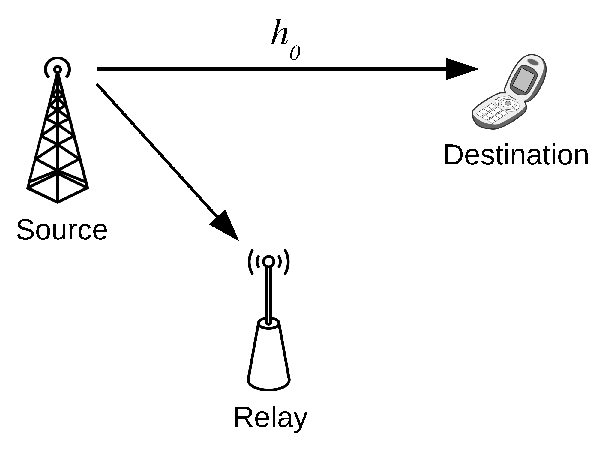
\includegraphics[width=4.0cm]{./figs/relayHARQ1.eps}}
      \centerline{(a) Phase 1}\medskip
    \end{minipage}
    \hfill
    \begin{minipage}[b]{.48\linewidth}
      \centering
      \centerline{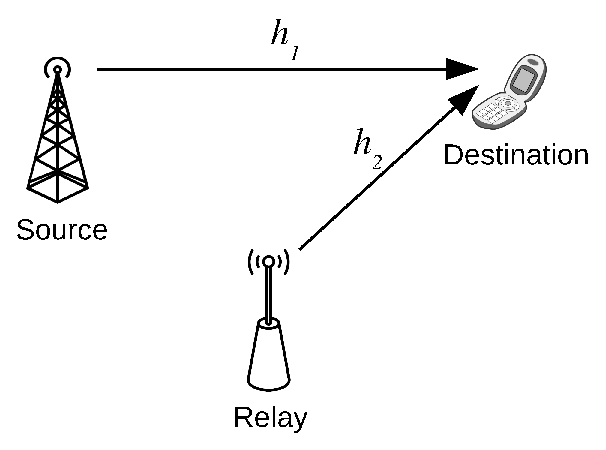
\includegraphics[width=4.0cm]{./figs/relayHARQ2.eps}}
      \centerline{(b) Phase 2}\medskip
    \end{minipage}
    \caption{Cooperative relay-HARQ networks.}
    \label{fig:system_model}
\end{figure}

The rest of this paper is organized as follows. Section~\ref{sec:model}
describes the cooperative relay-HARQ system model. Section~\ref{sec:core}
formulates the CoRe design into a Q3AP solution and provides a brief description
of the numerical algorithm. The numerical results are presented in
Section~\ref{sec:simulation}. Finally, Section~\ref{sec:conclusion} concludes
the paper.
%\hfill mds

\section{System Model and Problem Formulation}
\label{sec:model}
% Cooperative relay-HARQ channel 
We consider the cooperative relay-HARQ network depicted in
Fig.~\ref{fig:system_model}. Denote $\mathcal{C}$ as the constellation used by
this relay network. In the first phase, the source convert a bit
sequence of length $\log_2|\mathcal{C}|$ into symbols with Gray
mapping $\psi_0:
\{0,\ldots,|\mathcal{C}| - 1\}\rightarrow \mathcal{C}$. The bit sequence is
indexed by its decimal equivalence $p\in \{0,\ldots,|\mathcal{C}| - 1\}$.
Then the source transmit $\psi_0[p]$ to the destination via channel $h_0$
which is also overheard by the decode-and-forward (DF) relay.
We assume that relay is placed strategically so that it has
negligible decoding error rate as in~\cite{}. Upon receiving a request for
retransmission, the second phase is started. This time the source and the relay
adop remap $p$ into $\psi_1[p]$ and $\psi_2[p]$, respectively, where potentially
$\psi_1\not=\psi_0$ and $\psi_2\not=\psi_0$. The remapped symbols are
transmitted simultaneously on the same band to the destination via channel $h_1$
and $h_2$. In summary, the received signal at the destination
during the 2 phases are
\begin{subequations}
    \begin{align}
       y_1 & = h_0\psi_0[p] + v_1 \\
       y_2 & = h_1\psi_1[p] + h_2\psi_2[p] + v_2
    \end{align}
\end{subequations}
where $v_1\sim\mathcal{CN}(0,\sigma_v^2)$ and
$v_2\sim\mathcal{CN}(0,\sigma_v^2)$ are the additive noise. Thoughout this work,
we assume the channels $h_0$, $h_1$ and $h_2$ follows independent Rician
distribution.

% ML demodulator
Assuming that the destination has perfect channel state information (CSI), it
decides the index $p$ with the maximum likelihood (ML) rule
\begin{align}
    \min_{\hat{p}} |y_1 - \hat{h}_0\psi_0[\hat{p}]|^2 + |y_2-
    \hat{h}_1\psi_1[\hat{p}] - \hat{h}_2\psi_2[\hat{p}]|^2.
    \label{eq:ML}
\end{align}

% An example of a floating figure using the graphicx package.
% Note that \label must occur AFTER (or within) \caption.
% For figures, \caption should occur after the \includegraphics.
% Note that IEEEtran v1.7 and later has special internal code that
% is designed to preserve the operation of \label within \caption
% even when the captionsoff option is in effect. However, because
% of issues like this, it may be the safest practice to put all your
% \label just after \caption rather than within \caption{}.
%
% Reminder: the "draftcls" or "draftclsnofoot", not "draft", class
% option should be used if it is desired that the figures are to be
% displayed while in draft mode.
%
%\begin{figure}[!t]
%\centering
%\includegraphics[width=2.5in]{myfigure}
% where an .eps filename suffix will be assumed under latex, 
% and a .pdf suffix will be assumed for pdflatex; or what has been declared
% via \DeclareGraphicsExtensions.
%\caption{Simulation Results}
%\label{fig_sim}
%\end{figure}

% Note that IEEE typically puts floats only at the top, even when this
% results in a large percentage of a column being occupied by floats.


% An example of a double column floating figure using two subfigures.
% (The subfig.sty package must be loaded for this to work.)
% The subfigure \label commands are set within each subfloat command, the
% \label for the overall figure must come after \caption.
% \hfil must be used as a separator to get equal spacing.
% The subfigure.sty package works much the same way, except \subfigure is
% used instead of \subfloat.
%
%\begin{figure*}[!t]
%\centerline{\subfloat[Case I]\includegraphics[width=2.5in]{subfigcase1}%
%\label{fig_first_case}}
%\hfil
%\subfloat[Case II]{\includegraphics[width=2.5in]{subfigcase2}%
%\label{fig_second_case}}}
%\caption{Simulation results}
%\label{fig_sim}
%\end{figure*}
%
% Note that often IEEE papers with subfigures do not employ subfigure
% captions (using the optional argument to \subfloat), but instead will
% reference/describe all of them (a), (b), etc., within the main caption.


% An example of a floating table. Note that, for IEEE style tables, the 
% \caption command should come BEFORE the table. Table text will default to
% \footnotesize as IEEE normally uses this smaller font for tables.
% The \label must come after \caption as always.
%
%\begin{table}[!t]
%% increase table row spacing, adjust to taste
%\renewcommand{\arraystretch}{1.3}
% if using array.sty, it might be a good idea to tweak the value of
% \extrarowheight as needed to properly center the text within the cells
%\caption{An Example of a Table}
%\label{table_example}
%\centering
%% Some packages, such as MDW tools, offer better commands for making tables
%% than the plain LaTeX2e tabular which is used here.
%\begin{tabular}{|c||c|}
%\hline
%One & Two\\
%\hline
%Three & Four\\
%\hline
%\end{tabular}
%\end{table}


% Note that IEEE does not put floats in the very first column - or typically
% anywhere on the first page for that matter. Also, in-text middle ("here")
% positioning is not used. Most IEEE journals/conferences use top floats
% exclusively. Note that, LaTeX2e, unlike IEEE journals/conferences, places
% footnotes above bottom floats. This can be corrected via the \fnbelowfloat
% command of the stfloats package.

\section{Optimal Constellation Rearrangement}
\label{sec:core}
In this section we first formulate the min-BER CoRe design into a Q3AP problem,
and explain the numerical approach to compute the input cost matrix to Q3AP
problem. Then we provide an efficient algorithm to solve the Q3AP solution.

\subsection{BER Maximization via Q3AP solution}
% Q3AP formulation 
Assume that the information-bearing index $p$ follows a uniform distribution,
the BER can be upper-bounded using pair-wise error probability (PEP)~\cite{}
\begin{align}
    P_{BER} = \sum_{p=0}^{Q - 1}\sum_{q=0}^{Q - 1}\frac{B[p,
    q]}{Q}P_{PEP}(q | p) \label{eq:P_BER}
\end{align}
where $B[p,q]$ is the Hamming distance between the binary representation of $p$
and $q$ and $P_{PEP}(q | p)$ is the probability for the ML decoder to prefer $q$
over $p$ when $p$ is actually transmitted. According to~(\ref{eq:ML}), we have
\begin{align}
    P_{PEP}(q | p) = P_{h_0,h_1,h_2,v_0,v_1}\{\delta(p,q,\psi_1,\psi_2) < 0\}
    \label{eq:P_PEP}
\end{align}
i.e. given indices $p, q$ and the remapping scheme $\psi_1$, $\psi_2$, the
probability of random variable $\delta<0$ evaluated over the random variables
$h_0,h_1,h_2,v_0,v_1$, and $\delta$ is defined as
\begin{align}
    \delta & = |h_0(\psi_0[p] - \psi_0[q]) + v_0|^2 - |v_0|^2 +\notag\\ 
    &
    |h_1(\psi_1[p] - \psi_1[q])+h_2(\psi_2[p] - \psi_2[q])+v_1|^2 -
    |v_1|^2.
    \label{eq:delta}
\end{align}
In order to formulate the Q3AP problem, we denote binary variable $x_{pij} = 1$
if $\psi_1[p] = \psi_0[i]$ and $\psi_2[p] = \psi_0[j]$ and $x_{pij} = 0$
otherwise.
Denote $\mathbf{x} = \{x_{pij}|p,i,j=0,\ldots,Q-1\}$, and the
constraint sets:
\begin{subequations}
    \begin{align}
        \mathcal{P} & = \left\{\mathbf{x}:\,\sum_{p=0}^{Q-1}x_{pij} = 1,
        x_{pij}\in\{0, 1\}\right\}
        \\
        \mathcal{I} & = \left\{\mathbf{x}:\,\sum_{i=0}^{Q-1}x_{pij} = 1,
        x_{pij}\in\{0, 1\}\right\}
        \\
        \mathcal{J} & = \left\{\mathbf{x}:\,\sum_{j=0}^{Q-1}x_{pij} = 1,
        x_{pij}\in\{0, 1\}\right\}.
    \end{align}
\end{subequations}
Then from~(\ref{eq:P_BER})(\ref{eq:P_PEP})(\ref{eq:delta}), the BER-minimization
CoRe scheme $\min_{\psi_1, \psi_2}P_{BER}$ can be reformulated as
\begin{align}
    & \min_{\mathbf{x}}\sum_{p=0}^{Q-1}\sum_{i=0}^{Q-1}\sum_{j=0}^{Q-1}
    \sum_{q=0}^{Q-1}\sum_{k=0}^{Q-1}\sum_{l=0}^{Q-1}c_{pijqkl}x_{pij}x_{qkl}
    \label{eq:Q3AP}\\
    & \mbox{s.t. } \mathbf{x}\in \mathcal{P}\cap\mathcal{I}\cap\mathcal{J}
    \notag
\end{align}
in which
\begin{align}
    c_{pijqkl} & = \frac{B[p, q]}{Q}P_{h_0,h_1,h_2,v_0,v_1}\{\delta(p,i,j,q,k,l)
    < 0\}
    \label{eq:cpijqkl}
\end{align}
\begin{align}
    \delta & = |h_0(\psi_0[p] - \psi_0[q]) + v_0|^2 - |v_0|^2 +\notag
    \\
    &
    |h_1(\psi_0[i] - \psi_0[k])+h_2(\psi_0[j] - \psi_0[l])+v_1|^2 -
    |v_1|^2.\label{eq:delta}
\end{align}

\subsection{Computation of the Pair-wise Symbol Rate}

% serial expansion method
In this section we focus on the computation of the parameters $\{c_{pijqkl}\}$
of Q3AP problem. According to~\ref{eq:cpijqkl}, the key to compute $c_{pijqkl}$
lies in the evaluation of $P_{h_0,h_1,h_2,v_0,v_1}\{\delta(p,i,j,q,k,l)$, i.e.
the CDF of random variable $\delta(p,i,j,q,k,l)$ as in~(\ref{eq:delta}). For the
general Rician channel assumption
$h_m\sim\mathcal{CN}(\mu_{h_m},\sigma_{h_m}^2), m=0,1,2$, we extend the method
in~\cite{} to compute $P_{h_0,h_1,h_2,v_0,v_1}\{\delta(p,i,j,q,k,l) < 0\}$:
\begin{align}
    & P_{h_0,h_1,h_2,v_0,v_1}\{\delta(p,i,j,q,k,l) < 0\} \notag \\
    & \approx \frac{1}{2v}\sum_{t=1}^v \Re\left\{\Phi_{\delta}(\xi +
    j\xi\tau_t)\right\} + \tau_t\Im\left\{\Phi_{\delta}(\xi +
    j\xi\tau_t)\right\}
    \label{eq:expansion}
\end{align}
where the moment generating function (MGF) $\Phi_{\delta}(\omega) =
\mathbb{E}_{\delta}[\exp(-\omega\delta)]$, $\tau_k = \tan((k - 1/2)\pi/v)$
and $\Re\{\cdot\}$, $\Im\{\cdot\}$ denotes the real and image part,
respectively. Parameter $\xi$ is selected to ensure convergence of the
integration and \cite{taricco2002exact} suggested to use $\xi = 1/4$. The size
$u$ of the expansion~(\ref{eq:expansion}) needs to be larger when $
P_{h_0,h_1,h_2,v_0,v_1}\{\delta(p,i,j,q,k,l) < 0\}$ is smaller in order to
maintain an acceptable numerical accuracy.

To compute $\Phi_{\delta}(\omega)$, denote Gaussian random vectors $\mathbf{z}_1
= [h_0, v_0]^T$, $\mathbf{z}_{2} = [h_1, h_2, v_1]^T$, such
that $\mathbf{z}_m\sim\mathcal{CN}(\bm{\mu}_m, \mathbf{\Sigma}_m)$, $m=1,2$,
where
\begin{align}
    \bm{\mu}_1 = [\mu_{h_0}, 0]^T,& \; \bm{\mu}_{2} = [\mu_{h_1}, \mu_{h_2},
    0]^T
    \\
    \mathbf{\Sigma}_1 = \mbox{diag}\left(\sigma_{h_0}^2, \sigma_v^2\right), & \;
    \mathbf{\Sigma}_2 = \mbox{diag}\left(\sigma_{h_1}^2, \sigma_{h_2}^2,
    \sigma_v^2\right)
\end{align}
Then~(\ref{eq:delta}) can be rewritten as $\delta = \mathbf{z}_1^H\mathbf{A}_1\mathbf{z}_1 + \mathbf{z}_{2}^H\mathbf{A}_{2}\mathbf{z}_{2}$, where
\begin{subequations}
    \begin{align}
        \mathbf{A}_1 & = \left[
            \begin{array}{cc}
                |e_{pq}|^2  & e_{pq}^* \\
                e_{pq} & 0
            \end{array}
        \right] \\
        \mathbf{A}_2 & = \left[
            \begin{array}{ccc}
            |e_{ik}|^2 & e_{ik}^*e_{jl} & e_{ik}^*
            \\
            e_{ik}e_{jl}^* & |e_{jl}|^2 & e_{jl}^*
            \\
            e_{ik} & e_{jl} & 0
        \end{array}
        \right]
    \end{align}
\end{subequations}
in which where $e_{ab} = \psi_0[a] - \psi_0[b]$. Then the MGF can be computed
as~\cite{schwartz1995communication}
\begin{align}
    \Phi_{\delta}(\omega) & = \sum_{m=1,2}
    \frac{\exp(-\omega\bm{\mu}_m^H\mathbf{A}_m(\mathbf{I} +
    \omega\mathbf{\Sigma}_m\mathbf{A}_m)^{-1}\bm{\mu}_m)}{\det(\mathbf{I} +
    \omega\mathbf{\Sigma}_m\mathbf{A}_m)}.
\end{align}


% special case of Rayleigh fading
When the Rician-fading channel reduces to Rayleigh-fading channel, i.e.
when $\mu_{h_m}=0, m = 0, 1, 2$ there is a simple upperbound of
$P_{h_0,h_1,h_2,v_0,v_1}\{\delta(p,i,j,q,k,l) < 0\}$ similar
to~\cite{seddik2008trans}. Note that
\begin{align}
    & P_{h_0,h_1,h_2,v_0,v_1}\{\delta(p,i,j,q,k,l) < 0\}  \notag \\
    & = \mathbb{E}_{h_0,h_1,h_2}
    \left\{Q\left(\sqrt{\frac{\left|h_0e_{pq}\right|^2
    + \left|h_1e_{ik} + h_2e_{jl}\right|^2}
    {2\sigma_v^2}}\right)\right\}
\end{align}
Applying the same relaxation as in~\cite{seddik2008trans}, we have
\begin{align}
    & P_{h_0,h_1,h_2,v_0,v_1}\{\delta(p,i,j,q,k,l) < 0\} \notag \\
    & \leq \frac{3\sigma_v^4}{\sigma_{h_0}^2|e_{pq}|^2 (\sigma_{h_1}^2|e_{ik}|^2
    +\sigma_{h_2}^2|e_{jl}|^2)}
    \label{eq:PEP_UB}
\end{align}
which is tight in high-SNR regime.
\subsection{Q3AP Solution}
% Description of the Q3AP solution methods

\section{Numerical Results}
\label{sec:simulation}
% Simulation settings
In this section we present the numerical results of CoRe under various channel
settings. In our simulation, all Rician channels are assume to have the same Rician parameter 
$K$. Also we assume that during the second phase, the phase of channel $h_1$ and $h_2$ can be 
aligned at the source and relay, respectively. Consequently, we define $\mu_{h_0} = \mu_{h_1} = \sqrt{K/(K + 1)}$, $\mu_{h_2}=a\sqrt{K/(K + 1)}$,  $\sigma_{h_0}^2 = \sigma_{h_1}^2 = 1/(K+1)$ and $\sigma_{h_2}^2 = a^2/(K+1)$, where $a\in \mathbb{R}$ represents the ratio between the amplitude of the line of sight (LOS) components of the relay-to-destination and the source-to-destination link. Throughout the simulation we consider 16-QAM constellation thus $Q=16$.
% BER-SNR different amplitude, K = 10

% BER-SNR different amplitude, K = 1

% BER-SNR different phase, K = 10

% BER-SNR different phase, K = 1

% BER mismatch

\section{Conclusion}
\label{sec:conclusion}




% conference papers do not normally have an appendix


% use section* for acknowledgement
%\section*{Acknowledgment}
%The authors would like to thank...





% trigger a \newpage just before the given reference
% number - used to balance the columns on the last page
% adjust value as needed - may need to be readjusted if
% the document is modified later
%\IEEEtriggeratref{8}
% The "triggered" command can be changed if desired:
%\IEEEtriggercmd{\enlargethispage{-5in}}

% references section

% can use a bibliography generated by BibTeX as a .bbl file
% BibTeX documentation can be easily obtained at:
% http://www.ctan.org/tex-archive/biblio/bibtex/contrib/doc/
% The IEEEtran BibTeX style support page is at:
% http://www.michaelshell.org/tex/ieeetran/bibtex/
\bibliographystyle{IEEEtran}
% argument is your BibTeX string definitions and bibliography database(s)
\bibliography{IEEEabrv,mybibfile}
%
% <OR> manually copy in the resultant .bbl file
% set second argument of \begin to the number of references
% (used to reserve space for the reference number labels box)
%\begin{thebibliography}{1}
%\bibitem{IEEEhowto:kopka}
%H.~Kopka and P.~W. Daly, \emph{A Guide to \LaTeX}, 3rd~ed.\hskip 1em plus
%  0.5em minus 0.4em\relax Harlow, England: Addison-Wesley, 1999.
%\end{thebibliography}




% that's all folks
\end{document}


